\subsection{Reinterpreting identity as indiscernibility}

We assume that we are given an identity relation $\approx$,
  which partitions the subject terms $S_G$ according to
  equation \ref{eq:equivalence_set}.

%\small
\begin{equation}
\label{eq:equivalence_set}
  \equivset{x}
=
  \setdef{
    y \in S_G
  }{
    \equivpair{x}{y}
  }
\end{equation}
%\normalsize

Identity can be defined as the smallest equivalence relation,
  i.e. the most fine-grained partition of $S_G$.
For reasoning purposes, mainly the fact that $\approx$
  is an equivalence relation counts.
As we saw in principle \ref{principle:indiscernibility_of_identicals},
  identity implies indiscernibility with respect to all properties.

We can generalize the notion of indiscernibility,
  by parameterizing the set of properties with respect to which
  indiscernibility is determined.
According to this generalization,
  resources $x$ and $y$ are indiscernible with respect to
  a set of properties $PO \subseteq P_G \times O_G$
  iff $\forall_{p \in P}(p(x) \leftrightarrow p(y))$ is the case.

It is important to note that every indiscernibility relation
  is also an equivalence relation (reasoning!),
  although not necessarily the smallest one.
Moreover, every indiscernibility relation defined over the domain $S_G$
  is also an identity relation,
  only over a different domain \cite{Quine1950}.\footnote{
    For instance, the set of properties
      ``has an income of $x$ euro's a month''
      for decimals $x$ do not identify people
      (since two people may have the same income),
      but it does identify income groups.
    }

We now reinterpret the identity relation $\approx$,
  as if it were an indiscernibility relation
  whose set of properties $PO$ is implicit.
Based on the identity relation,
  we can make the set of properties explicit
  so that $\approx$ becomes an indiscernibility relation.
Definition \ref{def:indiscernibility_properties} makes
  the properties relative to which terms $x_i$ are indiscernibile
  explicit.

\begin{definition}[Indiscernibility properties]
\label{def:indiscernibility_properties}
\begin{align}
  \indpo_{\approx}(\set{\range{x_1}{x_n}})
=
  \setdef{
    \pair{p}{o} \in P_G \times O_G
  }{\nonumber\\
    \bigwedge_{1 \leq i \leq n}
      \exists p_i \in \equivset{p},
        \exists o_i \in \equivset{o}(
          \triple{x_i}{p_i}{o_i} \in G
        )
% Alternatively, we can place the quantifies outside the conjunction:
%    \exists_{\range{p_1}{p_n} \in \equivset{p}},
%      \exists_{\range{o_1}{o_n} \in \equivset{o}}
%        \bigwedge_{1 \leq i \leq n} \triple{x_i}{p_i}{o_i} \in G
  }\nonumber
\end{align}
\end{definition}

\noindent Notice that in definition \ref{def:indiscernibility_properties}
  we close both the predicate terms $p$ and the object terms $o$
  under identity.
Performing these closured is important,
  since ``Berlin'' and ``Berlijn'' (i.e., the Dutch spelling of ``Berlin'')
  may denote identical resources, as may ``lives in'' and ``woont in''
  (i.e., the Dutch spelling of ``lives in'').
When being given data stating that ``Person $a$ lives in Berlin''
  ``Person $b$ woont in Berlijn'', $a = b$, $\text{Berlin} = \text{Berlijn}$,
  and $\text{lives is} = \text{woont in}$,
  we want to identify the permutations of
  $\set{\text{lives in},\text{woont in}}$ and
  $\set{\text{Berlin},\text{Berlijn}}$
  as the indiscernibility properties.

Using definition \ref{def:indiscernibility_properties},
  we can deduce that the indiscernibility properties for
  the identity pair $\pair{\text{Amsterdam}}{\text{Berlin}}$
  would contain (amongst many others) the properties
  ``is a city'', ``has more than 100,000 inhabitants'', and
  ``is located in Europe''.

In the above, we were interested in the properties that resources share
  with one other (e.g., being a city, having more than 500,000 inhabitants).
But we are also interested in the predicates that a set of resources shares.
This amounts to a simple abstraction of
  definition \ref{def:indiscernibility_properties},
  equating the sets of objects (closed under identity)
  and only returning the set of shared RDF predicate terms
  (see definition \ref{def:indiscernibility_predicates}).

\small
\begin{definition}[Indiscernibility predicates]
\label{def:indiscernibility_predicates}
\begin{align}
  \indp_{\approx}(\setrange{x_1}{x_n})
=
  \setdef{
    p \in P_G
  }{
    \exists_{\range{p_1}{p_n} \in \equivset{p}}(\nonumber\\
        \equivset{
          \setdef{
            o \in O_G
          }{
            \triple{x_1}{p_1}{o}
          }
        }
      =
        \ldots
      =
        \equivset{
          \setdef{
            o \in O_G
          }{
            \triple{x_n}{p_n}{o}
          }
        }
    )
  }\nonumber
\end{align}
\end{definition}
\normalsize

\noindent For the earlier example, we have the identity closure of
  ``lives in'' as the set of indiscernibility predicates
  for persons $a$ and $b$,
  and the identity closure of ``is a'', ``has more than $x$ inhabitants'',
  and ``is located in'' as the set of indiscernibility predicates for
  $\texttt{Amsterdam}$ and $\texttt{Berlin}$.



\subsection{Discerning the same}

In the previous section we saw that resources are \emph{indiscernible}
  with respect to $PO$ iff they cannot be told appart
  in a language that only contains the properties denoted by $PO$
  (the so-called indiscernibility properties).
In the same vein,
  and builing upon definition \ref{def:indiscernibility_predicates},
  we say that two pairs of resources are \emph{simi-discernible}
  iff their indiscernibility predicates $P \subseteq P_G$ are the same.

For example, the pair $\pair{\texttt{Amsterdam}}{\texttt{Berlin}}$
  is simi-discernible to the pair $\pair{\texttt{Nanjing}}{\texttt{Dalian}}$
  because both pairs have the same set of discernibility predicates,
  namely $\set{\texttt{is a},\texttt{has more than } x \texttt{ inhabitants},$
  $\texttt{is located in}}$.

When we look at the pairs that constitute (the extension of)
  an identity relation, we see that all identity assertions look the same.
But when we take the considerations of the previous section into account,
  we see that within a given identity relation
  there are pairs with different discernibility predicates.
Stating this formally,
  simi-discernibility is an equivalence relation on pairs of resources,
  and induces a partition of the cartesian product of the domain.
Definition \ref{def:simidiscernibility_relation} makes this concrete
  in terms of the earlier definitions.

\begin{definition}[Simi-discernibility relation]
\label{def:simidiscernibility_relation}
\begin{align}
  \equiv_{\indp_{\approx}}
=
  \setdef{
    \pair{\pair{x_1}{x_2}}{\pair{y_1}{y_2}} \in (S_G^2)^2
  }{\nonumber\\
    \indp_{\approx}(\set{x_1,x_2}) = \indp_{\approx}(\set{y_1,y_2})
  }\nonumber
\end{align}
\end{definition}



\subsection{Partitioning identity}

The members of the partition induced by $\equiv_{\indp_{\approx}}$
  are sets of resource pairs that share the same sharing properties.\footnote{
    We briefly reflect on our wording here.
    Within a pair, what is shared are properties,
      denoted by a pair of an RDF predicate term and an RDF object term
      (in that order).
    Between pairs, what is shared -- if something is shared -- are predicates,
      denoted by RDF predicate terms.
    So it is indeed correct to state that
      resource pairs which are simi-discernible,
      are themselves sharing properties.
  }

Notice that the partitioned pairs contain but are not limited to
  the identity pairs.
Therefore, for sets of simi-discernible pairs
  we have the following three possibilities:
  \begin{itemize}
    \item All pairs are identity pairs.
          This characterizes a consistently portion of the identity relation,
          since no simi-discernible pair is left out of this set.
    \item Some pairs are identity pairs.
          This characterizes a portion of the identity relation which is not
          applied consistently with respect to the simi-discernibility relation.
    \item No pairs are identity pairs.
          This charactizes a portion of the collection of pairs
          that is consistently kept out of the identity relation.
  \end{itemize}

\noindent Each member of the simi-discernibility partition that is not
  of the third kind, i.e. every set of pairs that contains some identity pair,
  can be though of as an identity sub-relation.
The simi-discernibility partition therefore gives us
  a partitioning of the identity relation
  into \emph{identity sub-relations}.
Each identity sub-relation can be described in terms of
  its discernibility predicates,
  i.e. in meaningful term that come from the domain vocabulary.

For instance, in the IIMB dataset there are some identical resources that
  share the property \verb|IIMBTBOX:spoken_in|, while other pairs share
  the property \verb|IIMBTBOX:form_of_government|.
As a matter of fact, the set of pairs of resources that are spoken in
  the same language are disjoint from the set of pairs of resources
  that have the same form of government,
  indicating identity according to different criteria.
In this example, one subset of the identity relation does not discern
  resources that are spoken in the same language, whereas another subset
  of the identity relation does not discern resources that have the same
  form of government.



\begin{comment}
Fig. 1 shows an example
  of a discernibility partitioning for a given identity relation.

We can thus identify subsets of an identity relation based on
  differences in the sets of properties relative to which
  the resource pairs that they consist of are
  (in)discernible from one another.
Identity of indiscernibility criteria provides
  another equivalence relation
  ($\approx_{\indp}$, def. \ref{def:indiscernibility_partition}),
  that partitions the identity relation $\approx$ into
  identity subrelations that characterize identity based on different
  indiscernibility criteria.

\begin{figure*}
\label{fig:iimb_example}
\centering
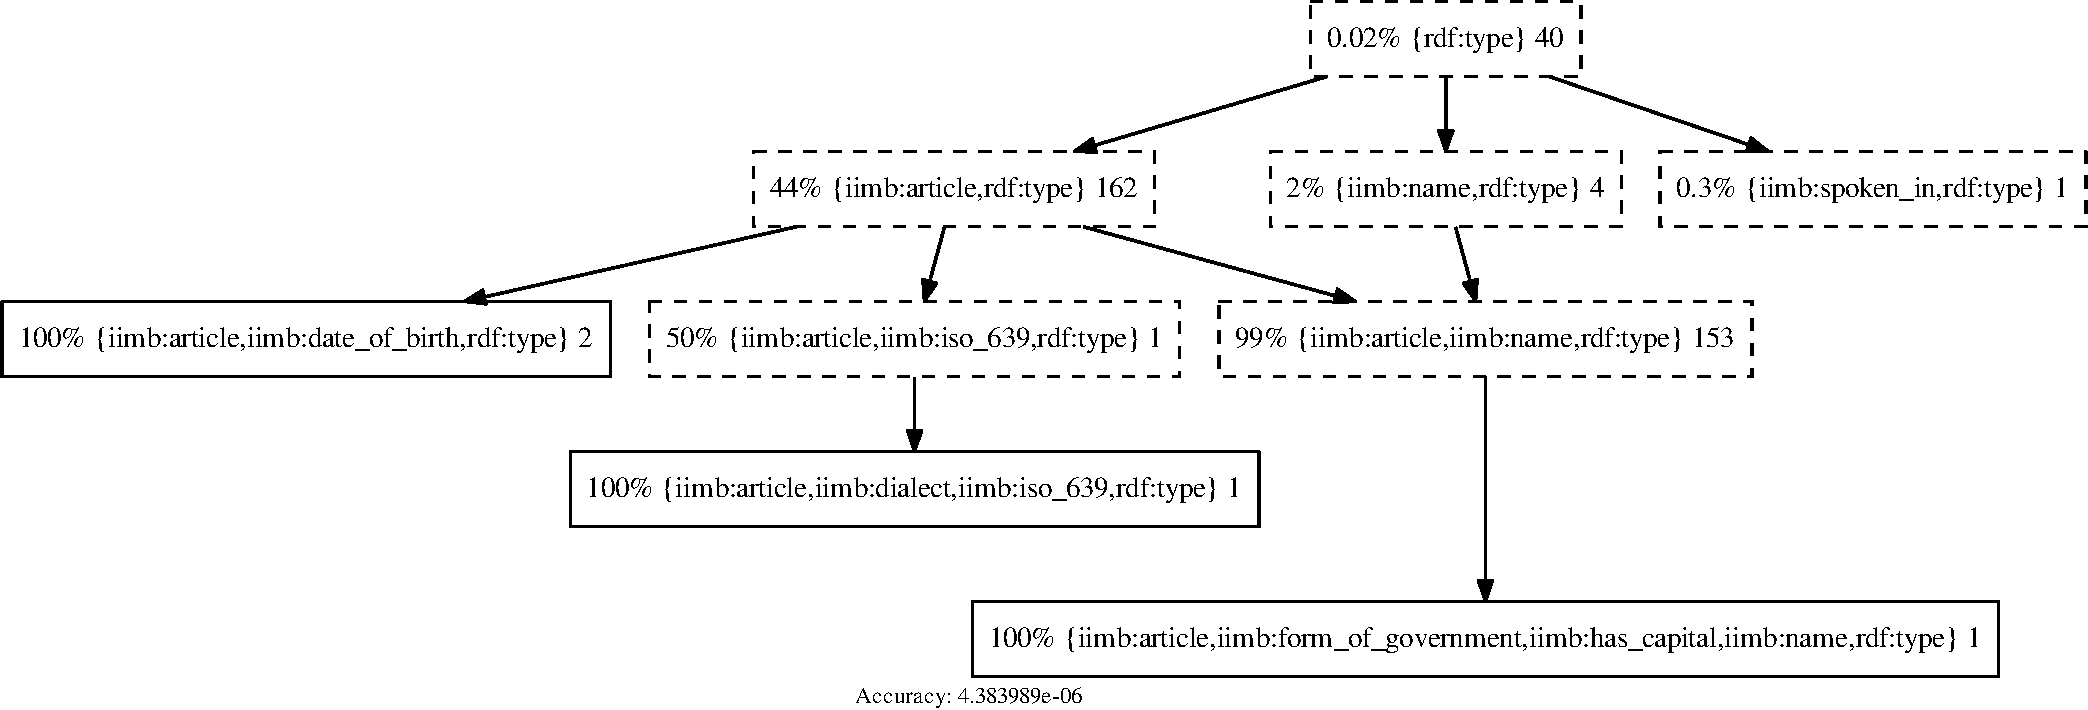
\includegraphics[width=\textwidth]{iimb_approximation_example_crop}
\caption{
  An example of a discernibility partition for an identity relation
    consisting of 365 pairs applied to the fourth IIMB linkset.
  Each node is annotated with the set of predicates $P$ for which
    its pairs are $P$-indiscernible.
  The number of identity pairs within each partition set
    is displayed to the right of the predicate set label.
  Partition sets that contain no identity pair are not show.
  The number that occurs to the left of the predicate label in each node
    indicates how may pairs in that node are identity pairs.
  The lower approximation consists of the nodes with a solid border,
    indicating that they contain only identity pairs.
  The higher approximation consists of all displayed nodes.}
\end{figure*}
\end{comment}

